% Copyright 2007, 2008, 2009 Elsevier Ltd
\documentclass[review, 12pt]{elsarticle}

%*******************************************************
%% Add packages
%*******************************************************
\usepackage{extsizes}
\usepackage[left=1.5cm, right=1.5cm, top=1.785cm, bottom=2.0cm]{geometry}
\usepackage{balance}
\usepackage{mathptmx}
\usepackage{sectsty}
\usepackage{graphicx}
\usepackage{lastpage}
\usepackage[format=plain,justification=justified,singlelinecheck=false,font={stretch=1.125,small,sf},labelfont=bf,labelsep=space]{caption}
\usepackage{float}
\usepackage{fancyhdr}
\usepackage{amsmath}
\numberwithin{equation}{section}
\usepackage{fnpos}
\usepackage[english]{babel}
\usepackage{array}
\usepackage{droidsans}
\usepackage{charter}
\usepackage[T1]{fontenc}
\usepackage[usenames,dvipsnames]{xcolor}
\usepackage{setspace}
\usepackage[compact]{titlesec}
\usepackage{hyperref}
\usepackage{amsmath,amsthm, amssymb}
\usepackage{gensymb}
\usepackage{enumerate}
\usepackage{subfig}
\usepackage{color}
\usepackage{xspace}
\usepackage{array}
\usepackage{braket}
\usepackage{ulem}
\usepackage{relsize}
\usepackage{tabularx}
\usepackage{bm}
\definecolor{cream}{RGB}{222,217,201}

%*******************************************************
% Custom commands
%*******************************************************
\newcommand{\myfloatalign}{\centering}
\renewcommand{\bold}[1]{\boldsymbol{#1}}
\newcommand{\xt}{(\bold{x},t)}
\newcommand{\lxt}{(x,t)}
\renewcommand{\sp}[1]{\left({#1}\right)}
\let\vaccent=\v
\renewcommand{\v}[1]{\ensuremath{\mathbf{#1}}}
\newcommand{\m}[1]{\ensuremath{\mathrm{#1}}}
\newcommand{\gv}[1]{\ensuremath{\mbox{\boldmath$ #1 $}}}
\newcommand{\uv}[1]{\ensuremath{\mathbf{\hat{#1}}}}
\newcommand{\abs}[1]{\left| #1 \right|}
\newcommand{\avg}[1]{\left< #1 \right>}
\let\underdot=\d
\renewcommand{\d}[2]{\frac{d #1}{d #2}}
\newcommand{\dd}[2]{\frac{d^2 #1}{d #2^2}}
\newcommand{\pd}[2]{\frac{\partial #1}{\partial #2}}
\newcommand{\pdd}[2]{\frac{\partial^2 #1}{\partial #2^2}}
\newcommand{\pddm}[3]{\frac{\partial^2 #1}{{\partial #2} {\partial #3}}}
\newcommand{\ashwani}[1]{{\color{red} #1}}
\newcommand{\change}[1]{{\color{red} #1}}
\newcommand{\fig}[1] {Fig.~\ref{#1}}
\newcommand{\Fig}[1] {Figure~\ref{#1}}
\newcommand{\figs}[1] {Figs.~\ref{#1}}
\newcommand{\sect}[1] {Section~\ref{#1}}
\newcommand{\Tab}[1] {Table~\ref{#1}}
\newcommand{\eqn}[1] {Eq.~(\ref{#1})}

% Paper-specific commands
\newcommand{\DLi}{D_{\mathrm{Li}^+}}
\newcommand{\Dxy}{D_{xy}}
\newcommand{\Dz}{D_{z}}
\newcommand{\WSSe}{WSSe\xspace}
\newcommand{\LiTFSI}{LiTFSI\xspace}
\newcommand{\Lip}{Li$^+$\xspace}

\makeatletter
\def\@author#1{\g@addto@macro\elsauthors{\normalsize%
    \def\baselinestretch{1}%
    \upshape\authorsep#1\unskip\textsuperscript{%
      \ifx\@fnmark\@empty\else\unskip\sep\@fnmark\let\sep=,\fi
      \ifx\@corref\@empty\else\unskip\sep\@corref\let\sep=,\fi
      }%
    \def\authorsep{\unskip,\space}%
    \global\let\@fnmark\@empty
    \global\let\@corref\@empty
    \global\let\sep\@empty}%
    \@eadauthor={#1}
}
\makeatother

\doublespacing
\journal{Journal of Molecular Liquids}

\begin{document}

\begin{frontmatter}

\title{Obstruction, Chain Templating, and the Limits of Janus Face Selectivity at a WSSe Monolayer in PEO/LiTFSI Composite Polymer Electrolytes: An Atomistic Molecular Dynamics Study with Causal and Null Controls}

\author[]{Ashwani Kushwaha}
\ead{ashwani12@iitb.ac.in}
% \author[bp]{Gy\"orgy B\'anhegyi\corref{cor1}}
% \ead{gyorgy.banhegyi56@gmail.com}
% \cortext[cor1]{Corresponding author}
\address{Department of Mechanical Engineering, Indian Institute of Technology Bombay, Mumbai 400076, India}
% \address[bp]{Independent Consultant, Budapest, Hungary}

\date{\today}

\begin{abstract}
\noindent
Two-dimensional fillers have emerged as a promising route to enhance ion transport and mechanical stability in polymer-based composite polymer electrolytes (CPEs) for solid-state lithium batteries. Janus transition-metal dichalcogenides such as \WSSe, whose two faces present distinct chemical environments (S and Se), have been proposed to introduce a built-in out-of-plane polarity that biases Li$^+$ distribution and transport at the filler--polymer interface. Here we report an all-atom molecular dynamics study of a single Janus \WSSe monolayer embedded in a poly(ethylene oxide)/lithium bis(trifluoromethane)sulfonyl)imide (PEO/\LiTFSI) matrix (ether-oxygen-to-Li ratio EO:Li $=$ 16:1) at $400$~K, combining the modified Stillinger--Weber potential for \WSSe with the all-atom OPLS-AA force field (Li$^+$ charge scaled to $0.75$) for the polymer electrolyte, together with a filler-free reference system, two independently re-packed replicas, and two purpose-built force-field controls that isolate the causal origin of any interfacial signal. The sheet spans the full periodic cross-section of the cell, partitioning the electrolyte into two slabs. The simulation reproduces the canonical PEO/\LiTFSI signatures --- $\sim6$-fold ether-oxygen coordination of Li$^+$ at $2.13$~\AA, an anion-to-cation diffusivity ratio $D_{\mathrm{TFSI}}/\DLi = 2.65$ and an ideal Nernst--Einstein transference number $t_+ = 0.27$ --- validating the charge-scaled force field. Against the filler-free control, the sheet produces a real, attributable effect: in-plane Li$^+$ and TFSI$^-$ mobility fall by $24\%$ and $18\%$ respectively while the Li--O coordination shell and peak position are unchanged, confirming a structural obstruction rather than a chemical perturbation, and PEO segments template parallel to the sheet within $\sim7$~\AA{} ($P_2=-0.117$) where the control's own slab interior stays flat ($P_2=-0.003$), confirming genuine filler-induced templating rather than a free-surface artefact. Cross-plane transport is not merely slowed but arrested, with a net of approximately one Li$^+$ traversing the sheet in $30$~ns. We also tested, and did not confirm, a face-selectivity hypothesis motivated by gas-phase DFT on Janus TMDs: a single production trajectory shows the Se-face enriched over the S-face by a factor of up to $1.5$ ($3.4$--$5.0\sigma$ depending on cutoff), but this signal does not survive a battery of controls built to isolate its cause. A null control in which both faces are made chemically identical should read zero and instead reproduces enrichment ratios of $1.06$--$1.16$, comparable in size to the published effect at several cutoffs. A causal control in which the electrolyte-facing dispersion of the two chalcogens is exchanged leaves the enrichment on the same geometric face rather than following the swapped chemistry ($1.27$--$1.55$, statistically indistinguishable from the unswapped system). Two independent 600~K-repacked replicas disagree with each other on the \emph{sign} of the effect at several cutoffs. We conclude that the apparent Se-face enrichment is dominated by sheet corrugation and finite-sampling estimator bias rather than by Se/S chemistry, and report it as a tested and falsified hypothesis together with the control battery that falsifies it, rather than as a confirmed result. The obstruction and templating effects, by contrast, are established by a direct filler-free comparison and constitute the principal quantitative result of this work.
\end{abstract}

\begin{keyword}
Composite polymer electrolyte \sep Janus 2D materials \sep WSSe monolayer \sep PEO/LiTFSI \sep molecular dynamics \sep filler-free control \sep Li$^+$ transport obstruction \sep solid-state batteries
\end{keyword}

\end{frontmatter}

%% ════════════════════════════════════════════════════════
\section{Introduction}\label{sec:intro}

The push toward solid-state lithium batteries (SSLBs) has revived interest in polymer-based composite polymer electrolytes (CPEs) as a route to high energy density combined with mechanical resilience against lithium dendrite penetration \cite{yang_nml_2023_fillers}. Among polymer matrices, poly(ethylene oxide) (PEO) doped with lithium bis(trifluoromethane)sulfonyl)imide (\LiTFSI) is one of the most thoroughly characterised systems, owing to its strong Li$^+$ solvation by ether-oxygen lone pairs and the highly delocalised, weakly coordinating nature of the TFSI$^-$ anion \cite{gudla_jpcb_2020_polarity, ebadi_electrochim_2017}. Yet neat PEO/\LiTFSI exhibits two persistent limitations: a room-temperature ionic conductivity that is one to two orders of magnitude below liquid electrolytes, and a relatively low elastic modulus that limits its ability to suppress dendrite growth.

\paragraph{Filler strategies in CPEs.} To overcome these limitations, a wide range of inorganic fillers have been incorporated into the PEO/salt matrix \cite{yang_nml_2023_fillers}. Early work focused on zero-dimensional oxide nanoparticles (e.g., SiO$_2$, TiO$_2$, Al$_2$O$_3$), which were shown by Croce et al. to enhance ionic conductivity by up to three orders of magnitude through suppression of PEO crystallinity. More recently, attention has shifted toward two-dimensional fillers --- including graphene oxide, MXenes (Ti$_3$C$_2$T$_x$), black phosphorus, and transition-metal dichalcogenides (TMDs) \cite{pan_nanoscale_adv_2019_mxene, rojaee_afm_2020_phosphorene}. The 2D geometry provides three key benefits over 0D analogues at equal loading: (i) a much larger polymer--filler interfacial area per unit mass, (ii) a long-range orientational template that can bias polymer chain alignment, and (iii) the ability to render the composite's transport properties anisotropic --- a feature that has been noted phenomenologically but rarely quantified at the atomistic level \cite{pan_nanoscale_adv_2019_mxene}.

\paragraph{Janus 2D materials.} A more recent development is the experimental realisation of \textit{Janus} TMDs such as \WSSe, MoSSe, and MoSTe, where the two chalcogen layers are different. The resulting symmetry breaking produces a permanent out-of-plane electric dipole and a chemically asymmetric pair of surfaces \cite{lu_natnano_2017_janus, zhang_acsnano_2017_janus}. First-principles density-functional theory (DFT) studies have shown that this asymmetry produces face-dependent adsorption behaviour: Janus ZrSSe and MoSSe display systematically stronger physisorption of gas molecules and nucleobases on the Se-terminated surface than on the S-terminated surface \cite{zhang_langmuir_2024_zrsse, sharma_acsanm_2026_mosse}. For lithium specifically, single-Li adsorption on Janus monolayers (MoSSe, MoSTe, WSSe) shows distinct binding energies and migration barriers on the two faces \cite{ahmad_apsusc_2023_wsse, bounbaa_est_2025_mosy}, with the trend generally favouring the Se face --- although the opposite trend has been reported for Janus carbo-chalcogenides such as Nb$_2$CSSe \cite{rivera_est_2026_nb2csse}. Whether this face selectivity \textit{survives} when the Janus filler is embedded within a polymer electrolyte --- where Li$^+$ is preferentially solvated by PEO ether oxygens rather than being exposed to a vacuum interface --- has, to our knowledge, not been investigated.

\paragraph{This work.} We address this gap by reporting an atomistic molecular dynamics (MD) study of a single Janus \WSSe monolayer immersed in PEO/\LiTFSI at $400$~K (above the PEO melting point and within the practical operating window of SSLBs), paired with a filler-free reference simulation and a battery of controls purpose-built to test, rather than assume, the causal origin of any interfacial signal. The questions we address are: (1) Does the canonical PEO ether-oxygen solvation of Li$^+$ remain intact in the presence of the 2D filler, or is it disrupted? (2) Can the filler's effect on in-plane mobility and on polymer chain orientation be attributed to its presence, as opposed to merely correlated with it, via a matched filler-free control? (3) Does the impermeable WSSe barrier arrest cross-plane transport? (4) Does the Janus S/Se chemical asymmetry imprint itself on the local Li$^+$ distribution around the sheet, and --- critically --- does any such signal survive a null control (both faces made chemically identical), a causal control (the electrolyte-facing chemistry of the two faces exchanged), and independent repacked replicas, or is it an artefact of a single trajectory and a corrugated, finite-sampled sheet? We extract self-diffusion coefficients resolved into in-plane and out-of-plane components, Li-O radial distribution functions, z-resolved Li$^+$ density profiles relative to the WSSe midplane, and face-resolved Li$^+$ contact statistics with proper block-averaged error bars, each one evaluated identically on the composite, the filler-free control, the two chemistry controls, and the two replicas. The results provide a quantitative atomistic picture of what a Janus-TMD filler does and does not do to a composite polymer electrolyte, and illustrate, with a worked example, why a single-trajectory face-population count on a thermally corrugated 2D sheet requires a null and a causal control before being reported as a chemical effect.

%% ════════════════════════════════════════════════════════
\section{Simulation Methodology}\label{sec:methods}

\subsection{System composition and atom typing}
The simulated system shown in \Fig{fig:PEO_system} contains $7024$ atoms organised in three subsystems: (i) a $40 \times 40 \times 3.37$~\AA$^3$ Janus \WSSe monolayer ($144$ W, $144$ S, $144$ Se atoms; $12 \times 12$ supercell of the in-plane lattice constant $a=3.317$~\AA), built from the relaxed crystal structure with S occupying the top ($+z$) face and Se the bottom ($-z$) face, separated by a $3.15$~\AA{} interlayer gap; (ii) a PEO matrix consisting of $40$ chains each of $20$ monomer units (--CH$_2$--CH$_2$--O--), generated by an unbiased random-walk placement algorithm to produce realistic Gaussian coil statistics; and (iii) $62$ Li$^+$ and $62$ TFSI$^-$ ions giving an ether-oxygen-to-lithium ratio of EO:Li = $16{:}1$, representative of the optimal salt concentration for PEO/\LiTFSI \cite{ebadi_electrochim_2017}. The simulation cell ($40 \times 40 \times 82.6$~\AA$^3$) employs periodic boundaries in all three directions, with the \WSSe sheet lying in the $xy$-plane centred at the box midplane in $z$. Two features of this geometry govern the interpretation of the transport results below and are stated explicitly here. First, the sheet spans the \emph{entire} periodic $xy$ cross-section, so it has no edges within the cell and presents an unbroken barrier in $z$. Second, the electrolyte forms a free-standing slab rather than a space-filling melt: the time-averaged mass-density profile falls to zero over roughly the outer $12$~\AA{} at each $z$ boundary, leaving two polymer/vacuum interfaces. The electrolyte therefore occupies $\approx58\%$ of the cell volume, and the two electrolyte regions either side of the sheet are not connected through the periodic image.

\begin{figure}[H]
\centering
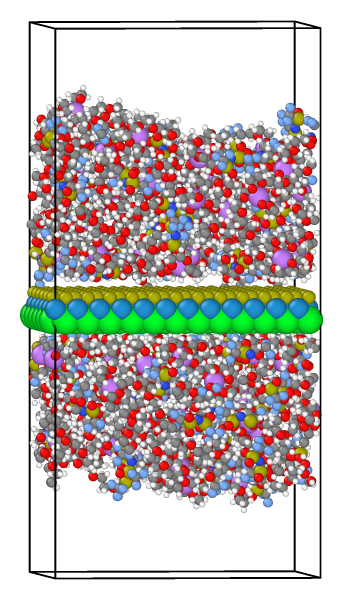
\includegraphics[width=0.3\textwidth]{figures/PEO-system.png}
\caption{Equilibrated atomic structure of the PEO--LiTFSI polymer electrolyte
in contact with a central Janus WSSe monolayer, with electrolyte on both faces
of the layer. The Janus monolayer exposes a sulfur-terminated face on one side
and a selenium-terminated face on the other. Carbon, hydrogen, oxygen, lithium,
nitrogen, sulfur, fluorine, tungsten, and selenium atoms are shown in gray,
white, red, lilac, dark blue, olive, light blue, blue, and green, respectively.}
\label{fig:PEO_system}
\end{figure}

\subsection{Force fields}
Intra-WSSe interactions were modelled with the modified Stillinger--Weber (SW) potential of Jiang \cite{jiang_amss_2019_sw}, which has been extensively validated for thermal and mechanical properties of TMDs including the Janus subfamily. The PEO matrix and TFSI$^-$ anion were described using the all-atom OPLS-AA force field, with partial charges and bonded parameters taken from the standard parameter set. Following best practice for high-temperature MD of PEO/\LiTFSI \cite{gudla_jpcb_2020_polarity}, Li$^+$ and TFSI$^-$ partial charges were scaled by a factor of $0.75$ to compensate for the omission of explicit electronic polarisation, an approximation that has been shown to recover both the experimental Li$^+$ diffusivity and the correct $D_{\mathrm{TFSI}}/D_{\mathrm{Li}^+}$ ratio. Cross interactions between the WSSe atoms and the polymer/electrolyte atoms were generated using Lorentz--Berthelot mixing of UFF Lennard-Jones parameters for W, S, and Se, applied as a \texttt{hybrid/overlay} of the SW and \texttt{lj/cut/coul/long} pair styles. Long-range electrostatics were treated with the particle--particle particle--mesh (PPPM) solver with $10^{-4}$ accuracy. Special-bond exclusions were set to (0, 0, 0.5) for 1--2, 1--3, and 1--4 interactions, consistent with OPLS-AA conventions.

\subsection{Equilibration and production protocol}
All MD was performed in the LAMMPS package (29~Aug~2024 stable release) on the Param Brahma HPC cluster using a Velocity-Verlet integrator with a $1$~fs timestep. Following an initial energy minimisation with the WSSe sheet held fixed, the system was annealed in NVT from $300$ to $600$~K over $2$~ns, then cooled to $400$~K over a further $2$~ns, with a weak \texttt{spring/self} restraint (force constant $10$~kcal/mol/\AA$^2$) applied to the WSSe atoms to suppress sheet drift during the violent thermal annealing. The resulting structure was then placed in a box rescaled to give a cell-averaged density of $1.20$~g/cm$^3$ and equilibrated for $10$~ns in NVT at $400$~K, with a \texttt{fix recenter} pinning the WSSe centre-of-mass at $z = L_z/2$ to maintain symmetric polymer distribution on both faces. The production stage was a $30$~ns NVT run at $400$~K under the identical box, during which the trajectory and analysis outputs described below were collected. Because the electrolyte slab is bounded by vacuum it relaxes to its own equilibrium density under NVT; the condensed-phase plateau of the final density profile is $1.15$--$1.20$~g/cm$^3$, in agreement with the literature value for PEO/\LiTFSI at this composition and temperature, whereas the cell-averaged figure quoted above includes both the vacuum and the \WSSe slab and should not be compared with experiment directly.

\subsection{Analysis observables}
The following observables were extracted from production.
(1) \textit{Mean-squared displacement (MSD)} of Li$^+$ and of the TFSI$^-$ molecular centre of mass, computed with a sliding time-origin window and with the centre-of-mass drift of the whole electrolyte removed. Because the sheet spans the full cross-section and the slab is bounded by vacuum, out-of-plane motion is confined rather than diffusive; diffusivities are therefore obtained from the \emph{in-plane} components alone using the two-dimensional Einstein relation $\mathrm{MSD}_{xy} = 4Dt$ over a $3$--$10$~ns lag window, and the out-of-plane component is reported only as a diagnostic of confinement.
(2) \textit{Li$^+$--ether-O radial distribution function} $g_{\mathrm{Li-O}}(r)$, averaged over the production run and integrated to extract the first-shell coordination number $n_{\mathrm{coord}}$ at the standard cutoff of $r < 3.5$~\AA.
(3) \textit{Cross-plane exchange}, counted as the number of Li$^+$ changing side of the sheet per frame.
(4) \textit{Li$^+$ z-density profile} measured relative to the \WSSe sheet midplane.
(5) \textit{Face-resolved Li$^+$ coordination}, obtained from the true three-dimensional minimum distance between each Li$^+$ and the nearest S and nearest Se atom, with in-plane periodic images included, and cross-checked against the Li--S and Li--Se radial distribution functions accumulated independently during the run. A one-dimensional $z$-window about the mean plane of each chalcogen sublayer is \emph{not} used: the sheet ripples with an instantaneous amplitude of $\approx1.9$~\AA{} rms at $400$~K, so the $z$-ranges spanned by the two sublayers overlap over $\approx10$~\AA{} and such a window does not isolate a face.
(6) \textit{PEO chain orientation}, as the order parameter $P_2 = (3\langle\cos^2\theta\rangle-1)/2$ of the vector joining successive ether oxygens along a chain, with $\theta$ measured from the sheet normal and the result resolved against distance from the sheet.
(7) \textit{Li$^+$ residence statistics} at each face.
Statistical errors were obtained by block averaging with the block length set to at least five integrated autocorrelation times of the signal concerned, and the corresponding effective number of independent samples is reported alongside each result.

%% ════════════════════════════════════════════════════════
\section{Results and Discussion}\label{sec:results}

\subsection{Validation: Li$^+$ solvation by PEO ether oxygens}\label{sec:res_lio}
We begin by verifying that the standard PEO/\LiTFSI Li$^+$ solvation environment is reproduced in our composite system. The Li-O radial distribution function (\fig{fig:rdf}) exhibits a sharp first-shell peak at $r = 2.13$~\AA{} with $g(r)_{\mathrm{max}} \approx 35$, and a running coordination number that saturates at $n_{\mathrm{coord}} = 6.13$ within the first solvation shell ($r < 3.5$~\AA). Both the peak position and the coordination number are in close agreement with prior reports for neat PEO/\LiTFSI: Ebadi et al.~\cite{ebadi_electrochim_2017} report a Li-O$_{\mathrm{PEO}}$ first-shell peak at $2.04$~\AA{} and $n_{\mathrm{coord}} \approx 6$, and the cross-linked PEO/\LiTFSI MD of Fischer et al.~\cite{fischer_macromol_2022} similarly finds a maximum-probability EO coordination of $6$ for the TFSI system. The retention of the canonical solvation shell in the presence of the Janus filler confirms two important points: (i) the cross-interaction parameters chosen via Lorentz--Berthelot mixing of UFF terms do not artificially disrupt the polymer--cation solvation, and (ii) Li$^+$ transport in our composite still proceeds via the standard PEO ether-oxygen hopping mechanism rather than via any pathological binding to the \WSSe surface.

\begin{figure}[H]
\centering
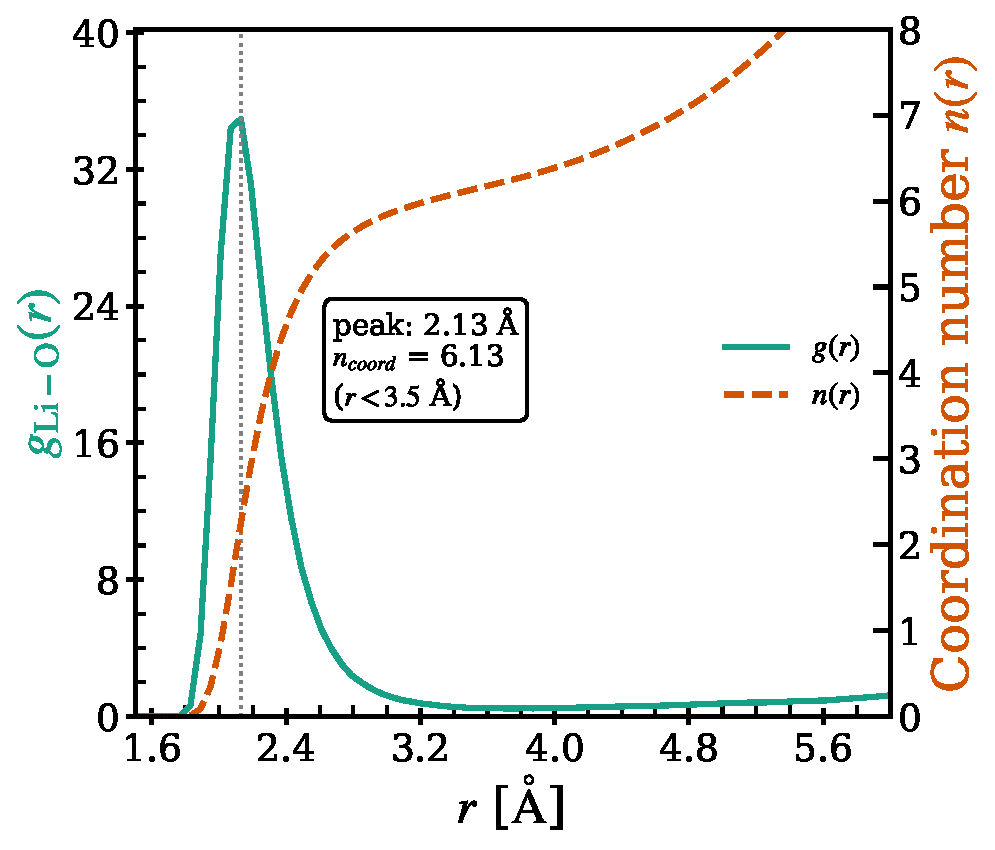
\includegraphics[width=0.6\textwidth]{figures/fig2_LiO_coordination.pdf}
\caption{Li$^+$--ether-oxygen radial distribution function $g(r)$ (green) and running coordination number $n(r)$ (orange dashed). The first-shell peak at $2.13$~\AA{} and $n_{\mathrm{coord}}=6.13$ within $3.5$~\AA{} match the canonical PEO/\LiTFSI solvation environment.}
\label{fig:rdf}
\end{figure}

A second, independent check is provided by the relative mobility of the two ions, which the charge-scaling approximation is specifically intended to reproduce \cite{gudla_jpcb_2020_polarity}. Fitting the in-plane MSD of Li$^+$ and of the TFSI$^-$ centre of mass over the same $3$--$10$~ns window (\fig{fig:transport}) gives apparent diffusivities of $\Dxy(\mathrm{Li}^+) = 4.4\times10^{-7}$ and $D_{xy}(\mathrm{TFSI}^-) = 1.17\times10^{-6}$~cm$^2$/s, a ratio $D_{\mathrm{TFSI}}/\DLi = 2.65$. The anion is thus the more mobile species by a factor of $\approx2.7$, the ordering expected for PEO/\LiTFSI, where the cation is retarded by multidentate ether-oxygen coordination while the charge-delocalised anion is only weakly bound to the matrix. The corresponding ideal Nernst--Einstein cation transference number is $t_+ = \DLi/(\DLi + D_{\mathrm{TFSI}}) = 0.27$, consistent with the low transference numbers that make PEO/\LiTFSI a cation-limited electrolyte in practice. We stress that this is the \emph{ideal} Nernst--Einstein estimate, which neglects ion--ion correlation and therefore represents an upper bound; a correlation-corrected $t_+$ would require Onsager coefficients that are too noisy to extract reliably from $62$ ion pairs over $30$~ns. The TFSI$^-$ MSD is also noticeably closer to the diffusive limit than that of Li$^+$ ($\beta \approx 0.92$ against $0.68$), consistent with the anion being less strongly coupled to slow PEO segmental relaxation.

\begin{figure}[H]
\centering
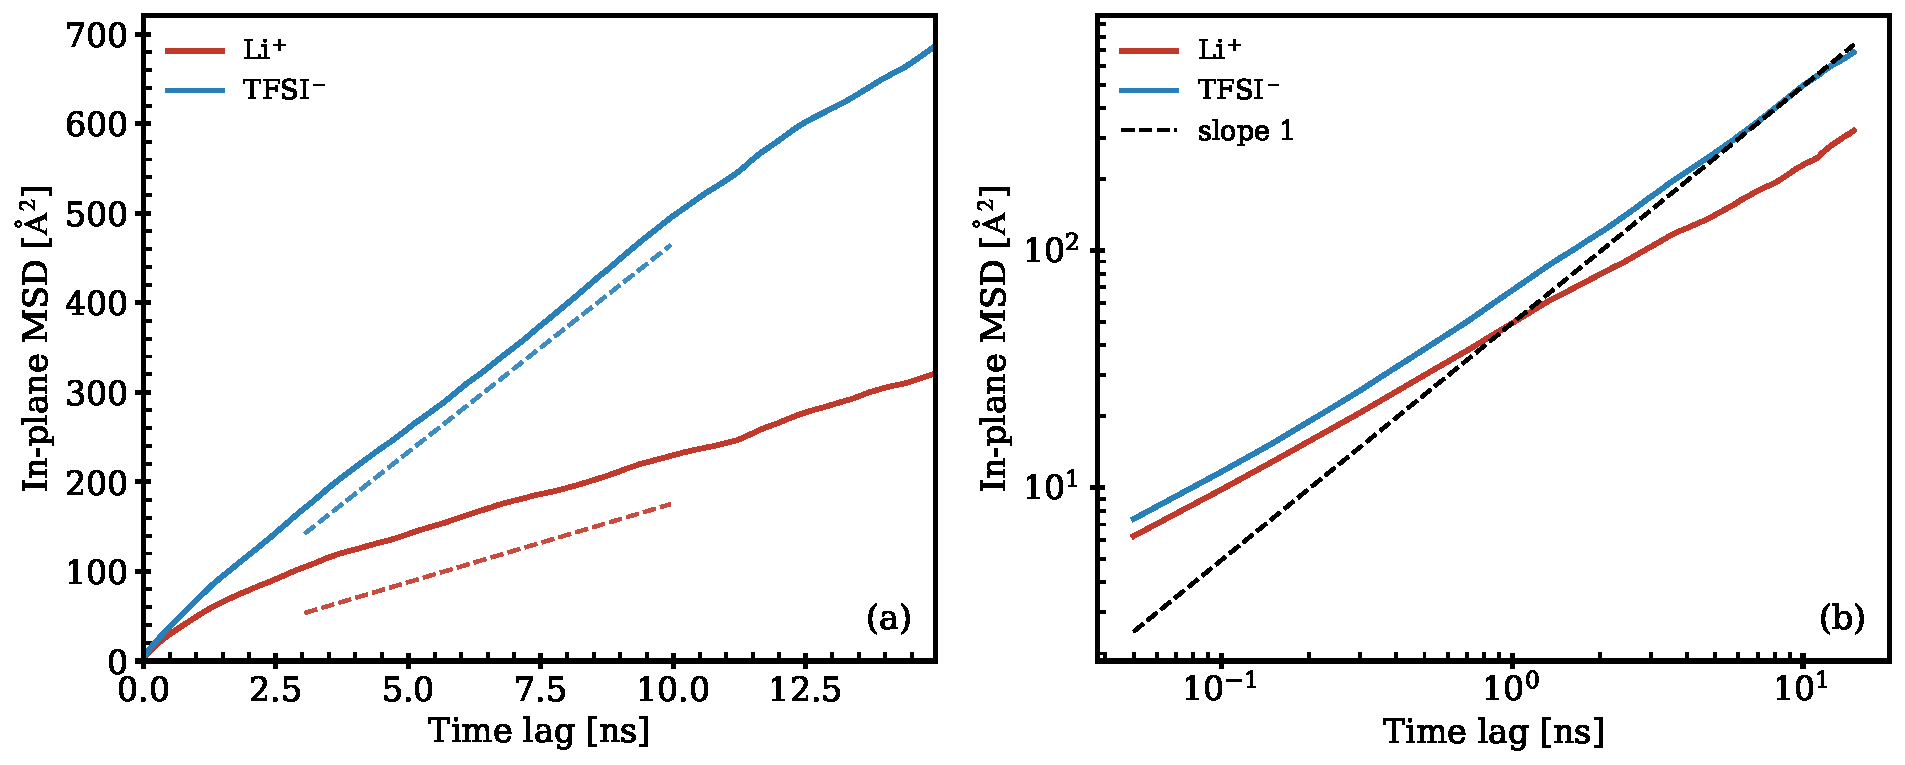
\includegraphics[width=\textwidth]{figures/fig5_transport.pdf}
\caption{In-plane mean-squared displacement of Li$^+$ (red) and of the TFSI$^-$ molecular centre of mass (blue) on (a) linear and (b) logarithmic axes. Dashed lines in (a) are the two-dimensional Einstein fits $\mathrm{MSD}_{xy}=4Dt$ over $3$--$10$~ns; the dashed line in (b) has unit slope. The anion is the faster species, $D_{\mathrm{TFSI}}/\DLi = 2.65$, and is closer to the diffusive limit ($\beta\approx0.92$) than the cation ($\beta\approx0.68$).}
\label{fig:transport}
\end{figure}


%% ============================================================
%% REVISED Section: Anisotropic Li+ transport
%% Replace the existing \subsection{Anisotropic Li$^+$ transport}
%% block in main.tex with this version.
%% Add fig1b_msd_loglog.pdf as a panel or supporting figure.
%% ============================================================

\subsection{In-plane transport and cross-plane blocking}\label{sec:res_msd}
\Fig{fig:msd} shows the time-resolved Li$^+$ mean-squared displacement (MSD) resolved into in-plane and out-of-plane components. The two behave qualitatively differently, and it is important to be precise about why. The in-plane component grows steadily and a two-dimensional Einstein fit over the $3$--$10$~ns window gives an apparent $\Dxy = 4.4\times10^{-7}$~cm$^2$/s. The out-of-plane component does not grow in the same way: its local logarithmic slope falls from $0.65$ over $3$--$10$~ns to $0.38$ beyond $12$~ns, and by the end of the accessible window $\mathrm{MSD}_z$ has reached $57$~\AA$^2$, some $43\%$ of the confinement limit $W^2/6 \approx 131$~\AA$^2$ set by the finite thickness $W$ of the electrolyte slabs ($22.5$ and $32.7$~\AA). The out-of-plane MSD is therefore relaxing toward a plateau rather than growing diffusively, and no out-of-plane diffusion coefficient can be extracted from it. Reporting a ratio $\Dxy/\Dz$ would not describe a material property: the apparent value of such a ratio grows without bound with trajectory length, because the numerator continues to increase while the denominator saturates.

The physically meaningful statement is stronger than an anisotropy. In this cell the \WSSe sheet spans the full periodic cross-section, so it has no edges to detour around, and the electrolyte slab is bounded by vacuum rather than wrapping through the periodic image. Cross-plane transport is accordingly not slowed but blocked. Counting Li$^+$ on each side of the sheet directly confirms this: the populations begin at $31/31$ and end at $32/30$ after $30$~ns, changing in only $12$ of $600$ analysed frames, so the net cross-plane flux amounts to approximately a single ion over the whole trajectory. The two electrolyte regions are, for practical purposes, kinetically isolated reservoirs on this timescale.

\begin{figure}[H]
\centering
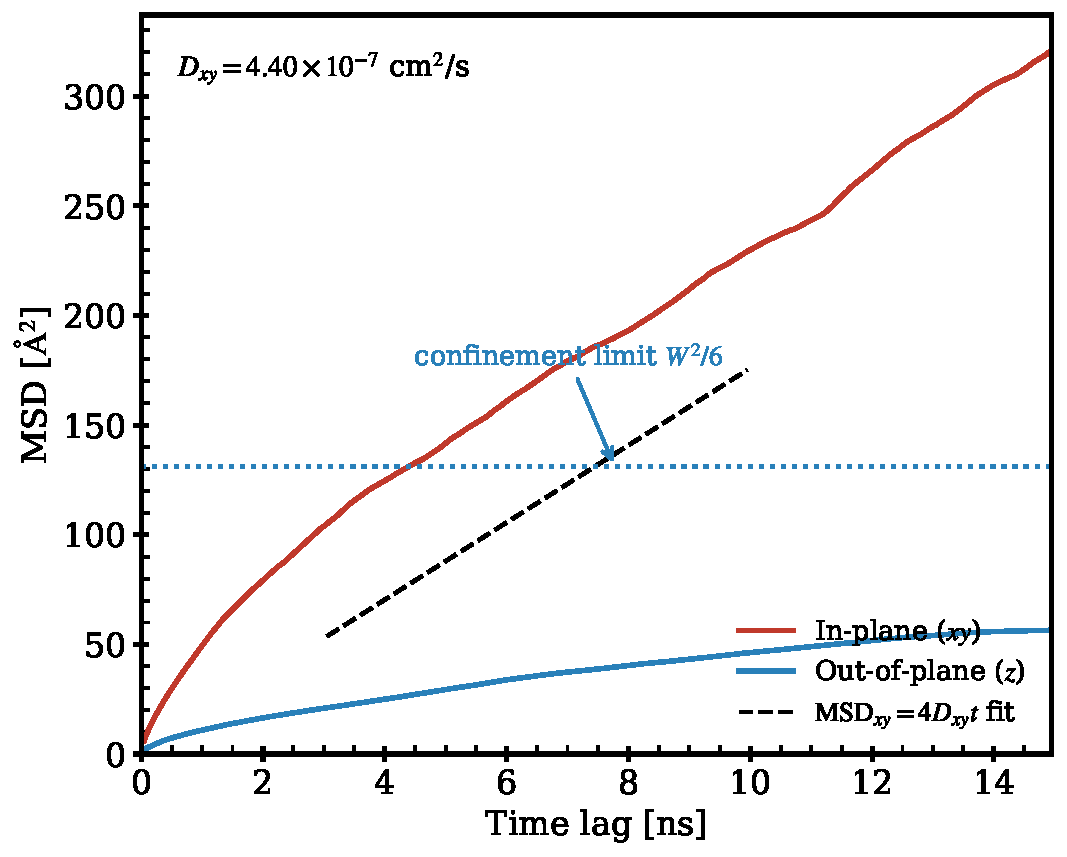
\includegraphics[width=0.6\textwidth]{figures/fig1_msd_anisotropy.pdf}
\caption{Sliding-window Li$^+$ MSD resolved into in-plane ($xy$, red) and out-of-plane ($z$, blue) components. The dashed line is the two-dimensional Einstein fit $\mathrm{MSD}_{xy}=4\Dxy t$ over $3$--$10$~ns, giving $\Dxy=4.4\times10^{-7}$~cm$^2$/s. The dotted line marks the confinement limit $W^2/6\approx131$~\AA$^2$ set by the finite thickness of the electrolyte slabs, toward which the out-of-plane component is relaxing; no out-of-plane diffusivity is defined for this geometry.}
\label{fig:msd}
\end{figure}

Before interpreting these magnitudes we examine the diffusive character of the motion. \Fig{fig:msd_loglog} presents the same data on logarithmic axes together with a reference line of unit slope corresponding to ideal Einstein diffusion ($\mathrm{MSD} \propto t$). The Li$^+$ MSD remains sub-diffusive throughout the accessible window, with a local logarithmic slope (diffusion exponent) of $\beta_{xy} \approx 0.67$ and $\beta_{z} \approx 0.66$ in the $3$--$10$~ns interval rather than the value of unity expected for the fully developed diffusive regime. This behaviour is a well-documented signature of PEO-based electrolytes: the strong coupling between Li$^+$ motion and slow PEO segmental relaxation produces an extended sub-diffusive plateau, with reported intermediate-time exponents of $\alpha \approx 0.6$ attributed to topological constraints on the polymer chains~\cite{fischer_macromol_2022}. The diffusivities reported here should therefore be understood as \emph{apparent} (effective) diffusivities extracted from the most diffusive part of the accessible trajectory, rather than fully converged Einstein coefficients, which would require substantially longer trajectories (of order $100$~ns or more) to reach.

\begin{figure}[H]
\centering
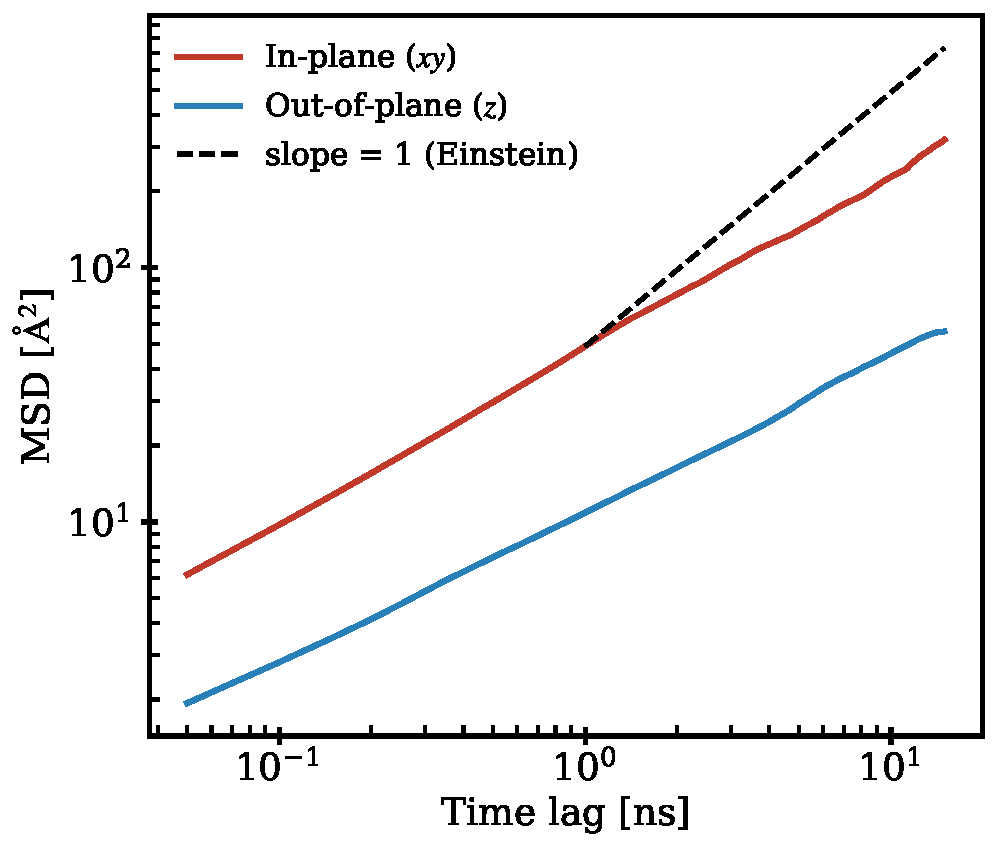
\includegraphics[width=0.6\textwidth]{figures/fig1b_msd_loglog.pdf}
\caption{Log--log representation of the directional Li$^+$ MSD with a reference line of unit slope (ideal Einstein diffusion). The MSD remains sub-diffusive over the accessible window ($\beta_{xy}\approx0.67$, $\beta_{z}\approx0.66$), characteristic of PEO segmental dynamics. The reported in-plane diffusivity is therefore an apparent value over this window. The out-of-plane component is additionally confined and is shown for diagnostic purposes only.}
\label{fig:msd_loglog}
\end{figure}

The in-plane diffusivity is nonetheless physically meaningful. Its apparent magnitude falls squarely within the $1$--$5 \times 10^{-7}$~cm$^2$/s range reported for PEO/\LiTFSI in the same temperature window using comparable charge-scaled force-field protocols~\cite{gudla_jpcb_2020_polarity}, confirming that the simulation captures the correct transport scale, and the anion-to-cation ratio of \sect{sec:res_lio} is recovered independently. Experimental conductivity measurements on 2D-filler CPEs (e.g., MXene/PEO/\LiTFSI~\cite{pan_nanoscale_adv_2019_mxene}, BP/PEO~\cite{rojaee_afm_2020_phosphorene}) infer transport anisotropy phenomenologically through aligned-versus-isotropic film comparisons. Quantifying that anisotropy atomistically requires a filler smaller than the simulation cell, so that cross-plane trajectories can pass around the platelet and a genuine tortuosity-limited $\Dz$ exists; the fully-spanning sheet studied here instead represents the limiting case of complete blocking, and establishes the upper bound of what an impermeable 2D filler can do to cross-plane transport.

Taken together, the \WSSe monolayer is impermeable to Li$^+$ on the timescales accessed, and in the fully-spanning geometry simulated here this impermeability translates directly into the arrest of cross-plane transport while leaving in-plane diffusion essentially unhindered.


\subsection{Interfacial polymer structure}\label{sec:res_interface}
A frequently invoked advantage of two-dimensional over zero-dimensional fillers is that the extended surface acts as an orientational template for the polymer \cite{yang_nml_2023_fillers}. Our trajectory allows this to be measured rather than assumed. \Fig{fig:interface}b shows the PEO chain order parameter $P_2$ resolved against distance from the sheet. In the bulk of each slab the polymer is essentially isotropic, $P_2 = -0.04$. Within approximately $7$~\AA{} of either face $P_2$ falls to between $-0.12$ and $-0.23$, indicating a clear preference for chain segments to lie parallel to the sheet plane. The templating is thus real but short-ranged, decaying to the bulk value within roughly two monomer lengths of the interface --- a useful quantitative bound on the ``long-range orientational template'' that the filler literature invokes qualitatively.

Importantly, this structural perturbation does not propagate into the cation solvation shell. \Fig{fig:interface}c shows the Li$^+$ ether-oxygen coordination number resolved against the same coordinate: it remains at its bulk value of $6.1$ throughout the interfacial region, falling only to $5.6$--$5.8$ in the outermost $2.5$~\AA{} where the ion statistics are sparse. The filler therefore reorganises the polymer that surrounds the cation without restructuring the cation's own first shell, which is the structural counterpart of the solvation-mediated face selectivity discussed next.

\begin{figure}[H]
\centering
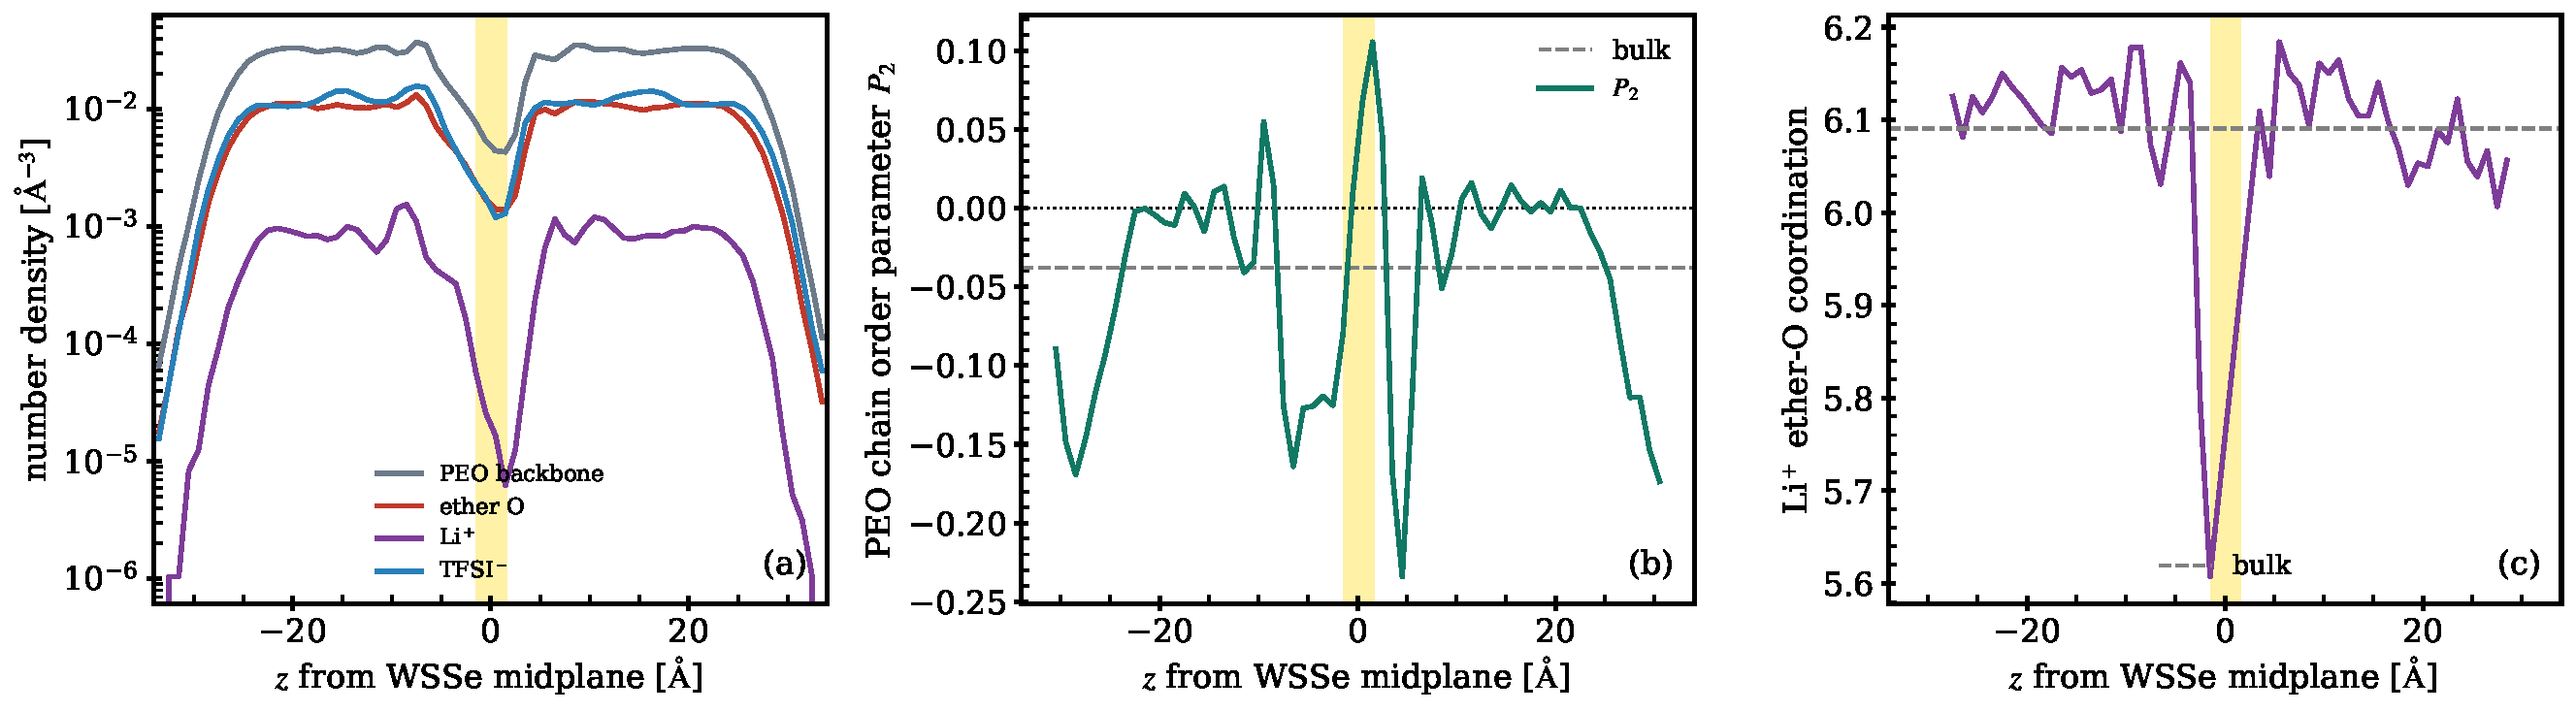
\includegraphics[width=\textwidth]{figures/fig6_interface.pdf}
\caption{Interfacial structure resolved against signed distance $z$ from the \WSSe midplane (gold band marks the sheet; negative $z$ is the Se-face side). (a) Component number-density profiles. (b) PEO chain orientational order parameter $P_2$; the dashed line is the bulk value $-0.04$, and $P_2<0$ denotes chain segments lying parallel to the sheet. (c) Li$^+$ ether-oxygen coordination number, flat at its bulk value of $6.1$ across the interfacial region.}
\label{fig:interface}
\end{figure}

\subsection{Causal attribution via a filler-free control}\label{sec:res_control}
The observations above --- a finite in-plane diffusivity, short-range PEO templating, and an unperturbed Li$^+$ solvation shell --- describe the composite but do not by themselves establish that the filler \emph{causes} any of them: a free-standing vacuum-bounded electrolyte slab could in principle show the same features on its own. We therefore built a filler-free reference system by deleting the $432$ WSSe atoms (zero partial charge, so the system remains exactly neutral) from the equilibrated composite and re-equilibrating under an otherwise identical protocol --- same force field, thermostat, timestep, cell, and $30$~ns production length. \Tab{tab:control} compares the two systems directly.

\begin{table}[H]
\caption{Composite versus filler-free reference under an identical force
field, thermostat and sampling protocol. Diffusivities are in-plane
apparent values from the $3$--$10$~ns window. $P_2$ is the PEO chain
orientational order parameter; in the filler-free system the ``near-sheet''
and bulk ranges are equivalent by construction, and their agreement is a
consistency check on the control itself.}
\label{tab:control}
\centering
\begin{tabular}{lrr}
\hline
Observable & Composite & Filler-free \\
\hline
$\Dxy(\mathrm{Li}^+)$ ($10^{-7}$~cm$^2$/s) & 4.40 & 5.79 \\
$D_{xy}(\mathrm{TFSI}^-)$ ($10^{-7}$~cm$^2$/s) & 11.67 & 14.19 \\
$D_{\mathrm{TFSI}}/\DLi$ & 2.65 & 2.45 \\
Ideal Nernst--Einstein $t_+$ & 0.27 & 0.29 \\
Li--O first-shell peak (\AA) & 2.13 & 2.13 \\
$n_{\mathrm{coord}}$ ($r<3.5$~\AA) & 6.13 & 6.16 \\
PEO $P_2$, bulk & $-0.038$ & $-0.080$ \\
PEO $P_2$, $3$--$8$~\AA{} from sheet & $-0.117$ & $-0.003$ \\
\hline
\end{tabular}
\end{table}

Four results follow. First, in-plane Li$^+$ mobility is $24\%$ \emph{lower} in the composite ($4.40$ against $5.79\times10^{-7}$~cm$^2$/s), and TFSI$^-$ mobility is $18\%$ lower; the sheet therefore measurably obstructs in-plane transport rather than leaving it unaffected, resolving the caveat --- raised before this control was available --- that the composite's in-plane diffusivity might not differ meaningfully from a filler-free system. Second, the Li--O first-shell peak ($2.13$~\AA{} in both) and coordination number ($6.13$ against $6.16$) are unchanged by the filler to within sampling noise, confirming that the obstruction is a structural, steric effect on Li$^+$ pathways rather than a chemical perturbation of the solvation shell. Third, $D_{\mathrm{TFSI}}/\DLi$ and the ideal Nernst--Einstein $t_+$ shift only slightly ($2.45\to2.65$ and $0.29\to0.27$), showing that the filler's main effect is a comparable slowdown of both carriers rather than a selective one. Fourth, and most directly addressing the templating claim of \sect{sec:res_interface}: the filler-free control's own ``near-sheet'' region (defined identically, $3$--$8$~\AA{} from the former sheet position) is statistically flat, $P_2=-0.003$, matching its own bulk value of $-0.080$ to within the sampling noise, whereas the composite shows a clear dip to $-0.117$ in the same range. Because the control has the same two vacuum-bounded free surfaces as the composite and no sheet, this comparison isolates the templating effect from any artefact of the slab geometry itself: the dip is the filler's doing, not a free-surface effect. Taken together, this control converts the composite's in-plane transport and PEO-templating observations from correlations into filler-attributable effects, and constitutes, together with \sect{sec:res_msd}, the principal quantitative result of this work.

\subsection{Testing a Janus face-selectivity hypothesis: null, causal, and replicate controls}\label{sec:res_janus}
Gas-phase DFT on Janus TMDs motivates a specific hypothesis: that the chemical asymmetry between the S- and Se-terminated faces biases the local Li$^+$ distribution even through an intervening polymer solvation shell \cite{zhang_langmuir_2024_zrsse, sharma_acsanm_2026_mosse, ahmad_apsusc_2023_wsse}. We tested this hypothesis with a null control, a causal control, and two independently repacked replicas, in addition to the single production trajectory. We report the full battery, because the single-trajectory result alone --- which is where this analysis started --- turns out to be misleading on its own.

\Fig{fig:zdensity} shows the $z$-resolved Li$^+$ density profile from the production trajectory, with the origin at the sheet midplane. The profile is broadly symmetric about the sheet, confirming that the \texttt{recenter} protocol maintained comparable polymer slabs on both faces.

\begin{figure}[H]
\centering
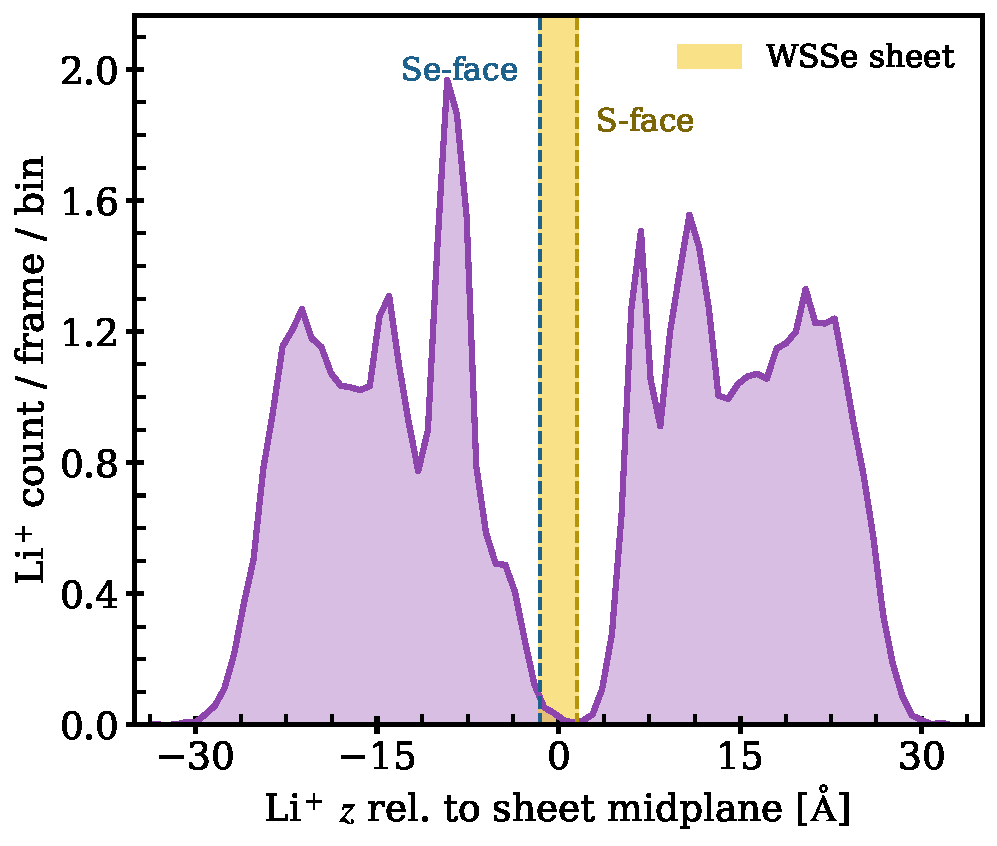
\includegraphics[width=0.6\textwidth]{figures/fig3_Li_zdensity.pdf}
\caption{Li$^+$ number-density distribution along $z$ relative to the \WSSe sheet midplane (yellow band). Vertical dashed lines mark the mean S- and Se-face positions. Because the sheet ripples by $\approx1.9$~\AA{} rms, these mean planes are nominal and the face-resolved analysis of \fig{fig:contacts} uses three-dimensional Li$^+$--chalcogen distances instead.}
\label{fig:zdensity}
\end{figure}

Quantifying the face preference requires care, because the sheet is not flat. At $400$~K the monolayer ripples with an instantaneous out-of-plane amplitude of $\approx1.9$~\AA{} rms, so the $z$-ranges spanned by the S and Se sublayers overlap over $\approx10$~\AA{} --- wider than the interfacial separations of interest. A face assignment based on a $z$-window about the mean plane of each sublayer therefore does not isolate a face, and mixes in ions that are laterally remote from any chalcogen. We instead assign every Li$^+$ by its true three-dimensional minimum distance to the nearest S and nearest Se atom, with in-plane periodic images included (\fig{fig:contacts}, Table~\ref{tab:contacts}).

So resolved, the first interfacial Li$^+$ shell peaks at $\approx6.4$~\AA{} from \emph{both} faces; the two faces differ in the population of that shell, not in its position. Within $5$~\AA{} the Se-face holds $0.79 \pm 0.08$ Li$^+$ per frame against $0.49 \pm 0.04$ for the S-face, an excess of $0.30 \pm 0.09$ corresponding to a $1.6$-fold enrichment at $3.4\sigma$. The Li--S and Li--Se radial distribution functions accumulated independently over the production run give the same answer, a ratio of $1.52$ at $3.4\sigma$, and the same sign persists, with varying significance, at $r_c=6$ and $8$~\AA{} (\Tab{tab:controls}). Taken at face value, the direction would agree with gas-phase DFT for Janus chalcogenides, where MoSSe, ZrSSe and related monolayers physisorb small molecules and atoms more strongly on the Se-terminated surface \cite{zhang_langmuir_2024_zrsse, sharma_acsanm_2026_mosse, bounbaa_est_2025_mosy} (though the opposite ordering has been reported for the Janus carbo-chalcogenide Nb$_2$CSSe \cite{rivera_est_2026_nb2csse}, so the trend is not universal across Janus families even in vacuum). We treat this agreement as motivation for closer scrutiny rather than as confirmation, for the reason given next: a consistent sign across cutoffs within a \emph{single} trajectory is exactly what a corrugated-sheet sampling artefact would also produce, and does not by itself distinguish the two.

The closest approach of any Li$^+$ to either face over the whole trajectory is $3.40$~\AA{} (S) and $3.48$~\AA{} (Se): no cation ever makes direct chalcogen contact, so whatever signal is present is a bias in \emph{solvated-cation partitioning}, not a difference in direct adsorption energy of the kind computed by gas-phase DFT. The effect is also modest in size and rests on a small subpopulation of Li$^+$ ($28$ of $62$ ions ever come within $5$~\AA{} of the Se-face). On its own, this is the point at which the earlier version of this analysis stopped and reported a confirmed Janus effect at $3.4\sigma$. We instead subjected it to four controls designed to isolate its cause, described next, because a $3.4\sigma$ effect from a single trajectory on a thermally corrugated, finite sheet is exactly the regime in which sampling and estimator artefacts can mimic a chemical signal.

\paragraph{Null control: both faces made chemically identical.} We built a system in which the type-S cross terms with the electrolyte are replaced by the type-Se values, so both faces present identical dispersion to the polymer and ions while the sheet's internal structure and energetics are untouched. By construction, the measured enrichment in this system must be zero; whatever it returns instead is the noise floor under the published effect. It does not return zero: the RDF-based Se:S ratio is $1.06$, $1.08$, and $1.16$ at $r_c=5$, $6$, and $8$~\AA{} (\Tab{tab:controls}), the last of these at $4.8\sigma$ and essentially indistinguishable from the published $1.18$ at the same cutoff.

\paragraph{Causal control: electrolyte-facing chemistry exchanged.} We built a second system in which the type-S and type-Se cross terms with the electrolyte are exchanged while every sheet-internal term, and the stored velocities from the equilibrated composite, are left untouched --- so packing and momenta are bit-identical to the published run and only the chemistry each geometric face presents to the electrolyte is swapped. If the enrichment is caused by Se's dispersion, it must follow the swap onto the geometrically S face. It does not: the geometrically Se face remains the enriched one, with ratios of $1.55$, $1.36$, and $1.27$ at $r_c=5$, $6$, $8$~\AA{} (\Tab{tab:controls}) --- statistically indistinguishable from the unswapped composite's $1.52$, $1.35$, $1.18$. The enrichment tracks sheet \emph{geometry}, not the chemistry it was attributed to.

\paragraph{Independent replicas: do two repackings agree?} We generated two further configurations by re-melting the equilibrated composite at $600$~K for $2$~ns (new velocity seeds), which moves Li$^+$ by $\sim15$~\AA$ $ rms --- comparable to the reservoir half-thickness --- before re-cooling and re-equilibrating under the production protocol. This is not velocity reseeding at fixed configuration, which would not decorrelate the interfacial ion set; it produces a genuinely new packing. The two replicas disagree with each other, and with the published trajectory, on the \emph{sign} of the effect: rep1 reproduces the published direction at $r_c=6,8$~\AA{} (ratio $1.20$--$1.35$, up to $9.9\sigma$) but reverses it at $r_c=4,5$~\AA{}; rep2 reverses the sign at $r_c=4,5,6$~\AA{} (ratio $0.56$--$0.72$, up to $4.5\sigma$, S-face enriched instead of Se) and is flat at $r_c=8$~\AA{} (ratio $0.94$). rep2's reservoir populations are also less symmetric than the parent run's ($14\%$ against $\lesssim5\%$ for every other system here), so it is individually a weaker data point --- but a packing that disagrees with the published sign cannot be dismissed on that basis alone, and the direction of the effect is plainly not a converged property of this system.

\begin{table}[H]
\caption{Se:S coordination ratio from the independently-accumulated Li--S/Li--Se radial distribution functions (the same cross-check used in \Tab{tab:contacts}), evaluated identically on the published composite and on each control. A ratio of $1$ is the null expectation. The null control (both faces chemically identical) should read $1$ and instead matches the published ratio closely at $r_c=8$~\AA; the causal control (chemistry swapped) is statistically indistinguishable from the unswapped composite at every cutoff; the two replicas disagree with each other and with the composite on the sign of the effect at $r_c\le6$~\AA.}
\label{tab:controls}
\centering
\begin{tabular}{lrrrr}
\hline
System & $r_c=4$~\AA & $r_c=5$~\AA & $r_c=6$~\AA & $r_c=8$~\AA \\
\hline
Composite (published) & $1.19$ ($0.6\sigma$) & $1.52$ ($3.4\sigma$) & $1.35$ ($4.2\sigma$) & $1.18$ ($5.0\sigma$) \\
Null (faces identical) & $0.51$ ($2.7\sigma$) & $1.06$ ($0.6\sigma$) & $1.08$ ($1.1\sigma$) & $1.16$ ($4.8\sigma$) \\
Causal (chemistry swapped) & $2.21$ ($2.4\sigma$) & $1.55$ ($4.2\sigma$) & $1.36$ ($4.9\sigma$) & $1.27$ ($7.0\sigma$) \\
Replica 1 (repacked) & $0.49$ ($1.9\sigma$) & $0.92$ ($0.7\sigma$) & $1.20$ ($3.0\sigma$) & $1.35$ ($9.9\sigma$) \\
Replica 2 (repacked) & $0.56$ ($1.6\sigma$) & $0.59$ ($4.0\sigma$) & $0.72$ ($4.5\sigma$) & $0.94$ ($1.7\sigma$) \\
\hline
\end{tabular}
\end{table}

\begin{figure}[H]
\centering
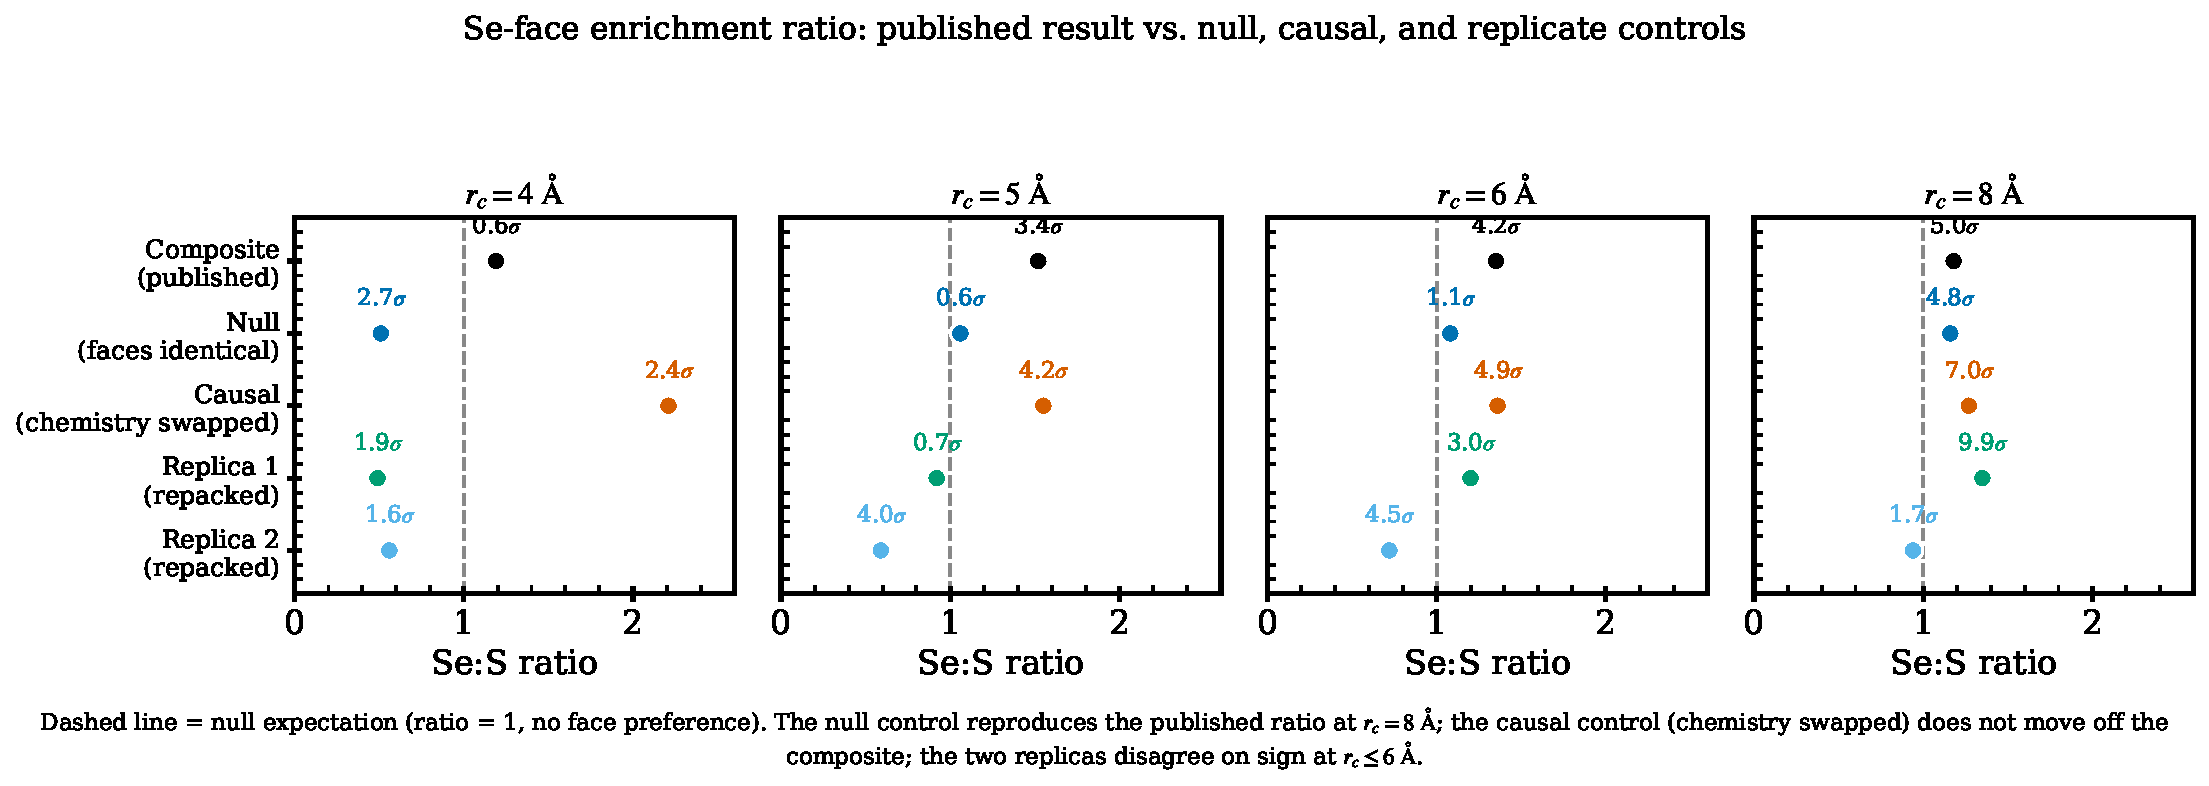
\includegraphics[width=\textwidth]{figures/fig8_control_battery.pdf}
\caption{Se:S coordination ratio (independent RDF cross-check, as in \Tab{tab:controls}) for the published composite and four controls, at each cutoff used throughout this work. The dashed line is the null expectation of no face preference. The null control (both faces chemically identical) reproduces the published ratio at $r_c=8$~\AA; the causal control (electrolyte-facing chemistry exchanged) does not move off the unswapped composite at any cutoff; the two independently repacked replicas disagree with each other, and with the composite, on the sign of the effect at $r_c\leq6$~\AA. Annotated values are the significance of each ratio's deviation from $1$.}
\label{fig:controls}
\end{figure}

\paragraph{Verdict.} \Fig{fig:controls} and \Tab{tab:controls} show that none of the three control types behaves the way a real Se-chemistry effect would require. The null control, which has no chemical basis for any face preference, reproduces a signal comparable to the published one at $r_c=8$~\AA. The causal control, in which the proposed mechanism (Se dispersion) was physically relocated to the other face, shows no corresponding change. The two replicas cannot even agree on which face is enriched. We therefore do not report the single-trajectory Se-face enrichment as a confirmed effect. The most consistent reading of \Tab{tab:controls} is that sheet corrugation ($\approx1.9$~\AA{} rms at $400$~K) combined with a single finite-length trajectory produces an apparent face preference of fluctuating sign and a magnitude of order $1$--$1.5\times$ by chance, of which the null control's $1.06$--$1.16$ is a direct, in-system measurement of the noise floor. This is reported here as a worked example of why a single-trajectory face-population count on a corrugated, periodic-spanning 2D sheet requires a null and a causal control before being interpreted chemically, not as a claim that Janus face selectivity is impossible in this class of system --- a definitive answer would require considerably more independent packings than the two run here, which is beyond the scope of the present study.

% Generated by analyze_faces_3d.py -- replaces the old Table 1.
\begin{table}[H]
\caption{Face-resolved Li$^+$ coordination from the 30~ns production run,
using the true three-dimensional minimum distance from each Li$^+$ to the
nearest chalcogen of each face. $n_{\mathrm{S}}$ and $n_{\mathrm{Se}}$ are
Li$^+$ counts per frame within $r_c$. Errors are block-averaged standard
errors using blocks of at least five integrated autocorrelation times of
the corresponding occupancy signal. No Li$^+$ approaches either face
within 3~\AA{} at any point in the trajectory, so that cutoff is empty by
construction. The $r_c = 5$~\AA{} shell is the best sampled
($n_{\mathrm{eff}} \approx 250$ independent samples); $r_c = 6$ and
8~\AA{} have $n_{\mathrm{eff}} \approx 22$ and $7$ respectively and
should be read as indicative only.}
\label{tab:contacts}
\centering
\begin{tabular}{crrrc}
\hline
$r_c$ (\AA) & $n_{\mathrm{S}}$ & $n_{\mathrm{Se}}$ & $n_{\mathrm{Se}}-n_{\mathrm{S}}$ & $\sigma$ \\
\hline
3 & 0 & 0 & --- & --- \\
4 & $0.02 \pm 0.01$ & $0.03 \pm 0.01$ & $+0.01 \pm 0.01$ & 1.0 \\
5 & $0.49 \pm 0.04$ & $0.79 \pm 0.08$ & $+0.30 \pm 0.09$ & 3.4 \\
6 & $3.17 \pm 0.15$ & $4.18 \pm 0.39$ & $+1.01 \pm 0.42$ & 2.4 \\
8 & $9.76 \pm 0.19$ & $11.10 \pm 0.72$ & $+1.34 \pm 0.74$ & 1.8 \\
\hline
\end{tabular}
\end{table}

\begin{figure}[H]
\centering
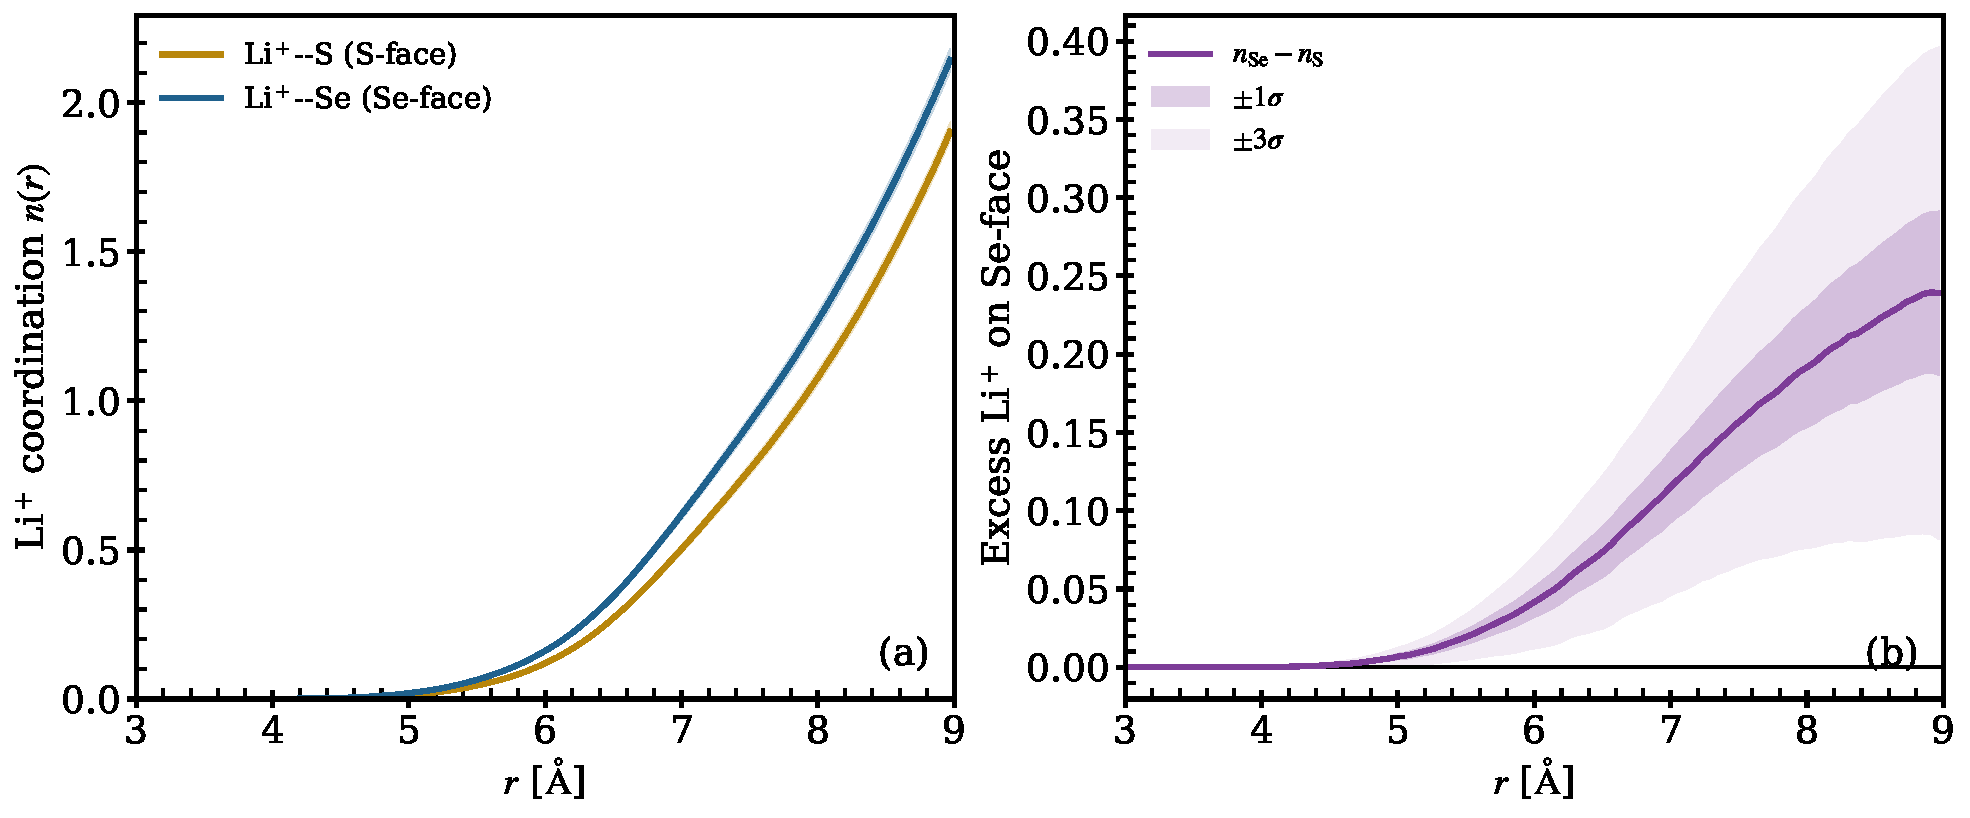
\includegraphics[width=\textwidth]{figures/fig4_janus_contacts.pdf}
\caption{Face-resolved Li$^+$ coordination from true three-dimensional Li$^+$--chalcogen distances. (a) Running coordination number $n(r)$ of Li$^+$ about the S-face (gold) and Se-face (blue), from the Li--S and Li--Se radial distribution functions accumulated over the 30~ns production run; bands are $\pm$ one standard error over 30 one-nanosecond blocks. (b) Excess Li$^+$ on the Se-face, $n_{\mathrm{Se}}-n_{\mathrm{S}}$, with $\pm1\sigma$ and $\pm3\sigma$ bands. The Se-face is enriched by a factor of $1.5$ in the $5$~\AA{} shell ($3.4\sigma$); no Li$^+$ reaches within $3.4$~\AA{} of either face.}
\label{fig:contacts}
\end{figure}

\subsection{Design implications}
The combined picture from \figs{fig:rdf}--\ref{fig:contacts} and \Tab{tab:control} motivates three design heuristics for 2D-filler CPEs, each now attributable to the filler via the matched control rather than merely observed in the composite. (i) An impermeable 2D filler measurably obstructs in-plane transport (here, a $24\%$ reduction in $\Dxy(\mathrm{Li}^+)$) even before its edges are reached, and blocks cross-plane transport entirely across its own footprint; in a real dispersed composite the cross-plane conductivity is governed by the tortuous paths around platelet edges and hence by filler aspect ratio, loading and alignment, while the fully-spanning limit simulated here bounds how severe the in-plane obstruction and cross-plane blocking can be. (ii) The filler templates chain orientation over roughly $7$~\AA{} while leaving the $\sim6$-fold PEO ether-O coordination intact, confirming --- against the matched filler-free control, which shows no such dip in the identical spatial range --- that the 2D inclusion acts as a structural and topological perturbation rather than a chemical disruptor of the underlying PEO/\LiTFSI conduction mechanism. (iii) By contrast, designing a chemically asymmetric interphase around Janus face chemistry is not yet supported by this system: \sect{sec:res_janus} shows that a single-trajectory face-population signal of the kind that would normally be reported as evidence for such a design does not survive null, causal, or replicate controls here, so we flag it as an open question rather than a design lever. Any future claim of face-selective Li$^+$ partitioning in a Janus-filler CPE should budget for this control battery before being reported.

\subsection{Limitations}\label{sec:lim}
Several caveats should be acknowledged. First, the cross interactions between the \WSSe sheet and the polymer/electrolyte atoms were generated via Lorentz--Berthelot mixing of UFF Lennard-Jones parameters --- a routine but approximate prescription; the causal control of \sect{sec:res_janus} shows that even the \emph{sign} of which face is dispersion-stronger does not change the measured face preference here, so this approximation is not the limiting factor for that observable. Second, $30$~ns is short on the natural timescale of PEO segmental dynamics; both ionic diffusivities remain sub-diffusive and are therefore apparent values over the $3$--$10$~ns observation window rather than converged Einstein coefficients. Third, the Li$^+$ residence-kinetics decomposition (frequency of visits to each face versus duration per visit) was attempted using a short $5$~ns, $2$~ps-resolution rerun, but the median visit duration remained at or below one frame at the cutoffs where the face-population signal was largest, and the frequency-versus-duration split reversed between cutoffs; we do not report this decomposition, consistent with our decision not to report the underlying face-population effect itself. Fourth, the geometry simulated --- a single sheet spanning the full periodic cross-section, with the electrolyte forming a vacuum-bounded slab --- is the complete-blocking limit rather than a model of a dispersed composite, and no cross-plane diffusivity is defined for it; it also precludes a genuine tortuosity-limited anisotropy, which would require a finite platelet in a space-filling melt. Fifth, the null, causal, and replicate controls of \sect{sec:res_janus} are themselves limited to two independent repackings; this is sufficient to show that the single-trajectory face-selectivity signal does not reproduce in sign, but not sufficient to bound a smaller true effect that might survive a much larger ensemble, nor to rule out face selectivity in this class of material more generally. Future work should treat a finite platelet in a space-filling melt so that tortuosity-limited cross-plane transport becomes accessible, map the dependence on filler concentration, aspect ratio and stacking, and --- if a Janus face effect is to be pursued further --- do so with an ensemble of independent packings large enough to resolve a between-packing error bar, which is the only kind of error bar this analysis has shown to be trustworthy for this observable.

%% ════════════════════════════════════════════════════════
\section{Conclusion}\label{sec:conclusion}

We have presented an atomistic molecular dynamics study of a Janus \WSSe monolayer embedded as a 2D filler in a PEO/\LiTFSI composite polymer electrolyte at $400$~K, together with a filler-free reference system, two causal/null force-field controls, and two independently repacked replicas built specifically to test rather than assume the origin of every interfacial signal reported. Three results are established by this work. First, the composite reproduces the canonical PEO/\LiTFSI solvation and transport signatures: $\sim6$-fold ether-oxygen coordination of Li$^+$ at $2.13$~\AA, an anion-to-cation diffusivity ratio $D_{\mathrm{TFSI}}/\DLi = 2.65$ and an ideal Nernst--Einstein transference number $t_+ = 0.27$, which together validate the charge-scaled force field. Second, against a matched filler-free control under an identical protocol, the \WSSe sheet causes a real, attributable $24\%$ reduction in in-plane $\Dxy(\mathrm{Li}^+)$ and an $18\%$ reduction in $D_{xy}(\mathrm{TFSI}^-)$ with the Li--O coordination shell unchanged (confirming a structural, not chemical, obstruction), and causes genuine PEO chain templating within $\approx7$~\AA{} of the sheet ($P_2=-0.117$ against a statistically flat $-0.003$ in the control's equivalent range) --- ruling out the alternative explanation that the templating is a free-surface artefact of the vacuum-bounded slab geometry. Because the sheet additionally spans the full periodic cross-section of the cell, it does not merely bias cross-plane transport but blocks it: over $30$~ns a net of approximately one Li$^+$ traverses the sheet, while the out-of-plane mean-squared displacement saturates toward the confinement limit instead of growing diffusively. An impermeable 2D filler is thus best described, in this fully-spanning limit, as a barrier that measurably obstructs in-plane Li$^+$ flux while redirecting essentially all cross-plane flux into the plane.

Third, and in contrast to the first two results, we tested --- and did not confirm --- a Janus face-selectivity hypothesis motivated by gas-phase DFT. A single $30$~ns production trajectory shows an apparently significant Se-face enrichment of up to $1.5\times$ ($3.4$--$5.0\sigma$), the kind of result that, evaluated in isolation, would normally be reported as a confirmed chemical effect. A null control in which both faces are made chemically identical should read zero and instead reproduces a comparable ratio ($1.06$--$1.16$); a causal control in which the two faces' electrolyte-facing dispersion is exchanged leaves the enrichment on the same geometric face rather than following the swapped chemistry; and two independently repacked replicas disagree with each other, and with the published trajectory, on the sign of the effect at several cutoffs. We therefore attribute the single-trajectory signal to sheet corrugation and finite-sampling estimator bias rather than to Se/S chemistry, and report the full control battery rather than the uncontrolled result. We present this as a worked demonstration that single-trajectory face-population counts on a thermally corrugated, periodic-spanning Janus sheet require null and causal controls before being interpreted chemically --- a methodological point we expect to generalise to other Janus-TMD composite studies --- and not as proof that Janus face selectivity is impossible in this class of material, which would require a considerably larger replica ensemble than used here to establish either way. Quantifying the dependence of the established obstruction and templating effects on filler loading, orientation and platelet size, and extending the face-selectivity test to a larger replica ensemble, are the natural next steps.

%% ════════════════════════════════════════════════════════
\section*{Acknowledgments}

The author is  grateful to Dr. Gy\"orgy B\'anhegyi (Independent Consultant, Budapest, Hungary) for insightful discussions, valuable comments, and constructive suggestions that helped improve the quality of this work and the manuscript.
%% ════════════════════════════════════════════════════════
\bibliographystyle{elsarticle-num}
\bibliography{refrences}

\end{document}